\documentclass[10pt]{article}
\usepackage[a4paper,margin=2cm]{geometry}
\usepackage{booktabs,longtable,amsmath,amssymb,graphicx,pdfpages,caption,lscape}
\captionsetup{font=small,labelfont=bf}
\title{\bfseries Two-Lagrangian CL inflow fits of the SPARC category-B galaxies:\\ detection, model selection, fit quality and robustness}
\author{Automated analysis for E.P.J.\ de Haas}\date{}
\begin{document}\maketitle
\section*{Summary}
Category B contains the 45 SPARC galaxies whose single-Lagrangian (single-L) CL residuals show a significant $+-+$ wave. For all of them the two-Lagrangian (two-L) model of Eqs.~(24)--(26) was fitted and compared with the single-L fit by BIC. In 23 galaxies the two-L description is accepted ($\Delta\mathrm{BIC}<-6$); in 22 the wave is real in sign but too weak to justify two extra parameters, and the single-L fit is kept. The accepted fits split into three groups. 13 are clean nested fits: physically ordered ($M_2>M_1$, no large drop at $R_2$) and statistically adequate. 5 are improved but still need more regions ($\chi^2_\nu>2$). 5 are not nested, meaning the fit exploits the discontinuity at $R_2$. For the clean nested fits the median RMS$_\mathrm{rel}$ in $v^2$ falls from 0.251 to 0.127 and the median Durbin--Watson statistic rises from 0.33 to 1.33. The outer scale is well determined ($\sigma_{v_{L2}}/v_{L2}$ = 1.6\%, $\sigma_{R_2}/R_2$ = 5\% from profile likelihood). The inner scale is less well determined ($\sigma_{M_1}/M_1$ = 22\%). Eight of the 13 galaxies identified as double fits in 2018 are recovered as clean nested fits. The main caveats are that $R_2$ is a discontinuity location, whose likelihood is non-smooth and in some galaxies multimodal, and that residual structure persists in 7 of the 13 clean fits, pointing to further (virial) regions.

\section{Sample and procedure}
\paragraph{Selection.} Category B was defined in the full-SPARC pipeline. After the single-L CL fit ($H_z=2.2\times10^{-18}\,\mathrm{s^{-1}}$, fits on $v^2$ with $\sigma_{v^2}=2V_\mathrm{obs}\delta V_\mathrm{obs}$), the weighted residuals must fail the one-sided runs test ($p_\mathrm{runs}<0.05$), agree to at least 80\% with a three-segment $+-+$ sign template, and agree better with it than with the reverse $-+-$ template.
\paragraph{Two-L model.} Eqs.~(24)--(26): bulge $r\le R_1$ and bar zone $R_1<r\le R_2$ governed by $L_1$ $(M_1,R_1)$, disk $r>R_2$ by $L_2$ $(M_2,R_2)$, with asymptotic speeds $v_{Li}=\sqrt{3/2}\,X_i$, $X_i=\sqrt{2GM_i/R_i}-H_zR_i$. A shared offset $\Phi_\mathrm{BH}$ is tested as a third variant.
\paragraph{Fitting and selection.} The two-L fit is seeded at $R_2=r_{\times1}/0.8$ (first $+\to-$ residual crossover) and cross-checked by a global grid and by the $R_2$ profile scan below; the best optimum is kept. A two-L fit is accepted if $\Delta\mathrm{BIC}=\mathrm{BIC_{2L}}-\mathrm{BIC_{1L}}<-6$ (strong evidence), and marked tentative when $n\le13$.
\paragraph{Uncertainties.} $M_1$, $R_1$, $M_2$: local covariance. $R_2$: because $v^2$ is discontinuous at $R_2$, $\chi^2(R_2)$ is piecewise smooth, changing slope whenever $R_2$ crosses a data radius, so the covariance error is unreliable. $R_2$ and $M_2$ are therefore given as profile-likelihood intervals ($\Delta\chi^2\le1$, other parameters refitted on a grid of 140 $R_2$ values). Jackknife: leave-one-out refits. Systematic: refits with distance $+\delta D$ and inclination $+\delta i$, added in quadrature. $H_z$ sensitivity: refit with $H_z=0$.
\paragraph{Post-hoc classification of accepted fits.} \textbf{Not nested (N)}: $M_2<M_1$ or $v^2$ drops by more than 40\% at $R_2$. \textbf{Needs more regions (M)}: $\chi^2_\nu>2$ after two-L. \textbf{Clean nested}: neither. Grades: \textbf{I} all four parameters within 30\% (profile errors for $R_2,M_2$), at least 2 points in bulge and bar zones and 3 in the disk, jackknife scatter $\le30\%$; \textbf{II} both $v_{L1}$ and $v_{L2}$ within 10\%; \textbf{III} otherwise.

\section{Model selection outcome}
\begin{table}[h]\centering\small\caption{Category-B outcome.}\begin{tabular}{lrl}\toprule Outcome & $N$ & Galaxies\\\midrule
Clean nested two-L, grade I & 6 & \parbox[t]{10.5cm}{\raggedright D631--7, DDO161, IC2574, NGC3741, NGC7793, UGC04278}\\
Clean nested two-L, grade II & 7 & \parbox[t]{10.5cm}{\raggedright ESO116--G012, F571--8, NGC0055, NGC0247, UGC00731, UGC07524, UGC12732}\\
Two-L, needs more regions (M) & 5 & \parbox[t]{10.5cm}{\raggedright DDO154, NGC1003, NGC2403, NGC5585, UGC03580}\\
Not nested (N) & 5 & \parbox[t]{10.5cm}{\raggedright NGC3726, NGC4013, UGC02885, UGC06614, UGC06787}\\
Single-L kept, $-6\le\Delta$BIC$<-2$ & 7 & \parbox[t]{10.5cm}{\raggedright NGC3109, NGC3972, NGC4010, UGC06446, UGC07125, UGC07323, UGC07399}\\
Single-L kept, $-2\le\Delta$BIC$<0$ & 3 & \parbox[t]{10.5cm}{\raggedright ESO079--G014, NGC4214, UGC05829}\\
Single-L kept, $\Delta$BIC$\ge0$ & 12 & \parbox[t]{10.5cm}{\raggedright F568--1, F568--3, F574--1, F579--V1, KK98--251, NGC0100, NGC2976, NGC5005, UGC08286, UGC08550, UGC12632, UGCA444}\\
\bottomrule\end{tabular}\end{table}
All 45 galaxies have significant single-L residual structure ($p_\mathrm{runs}<0.05$ by selection). The rejected galaxies differ from the accepted ones mainly in amplitude, not in shape. Their single-L fits are already good (median $\chi^2_\nu$ = 0.50, RMS$_\mathrm{rel}$ = 0.133, against 2.98 and 0.247 for the accepted ones), so the wave is coherent but lies within the SPARC errors. 12 of them have $\Delta\mathrm{BIC}\ge0$. Among these are F568-1, F574-1, F579-V1 and UGC 8286, which were single fits in 2018 as well. The seven galaxies with $-6\le\Delta\mathrm{BIC}<-2$ (positive but not strong evidence) include the 2018 double fits NGC 3109, NGC 3972 and UGC 6446. With $n=10$--25 points, a threshold of $-6$ is conservative for them, and they are the natural candidates for confirmation with more data. Their status is therefore \emph{undecided} rather than single-L.
\begin{figure}[h]\centering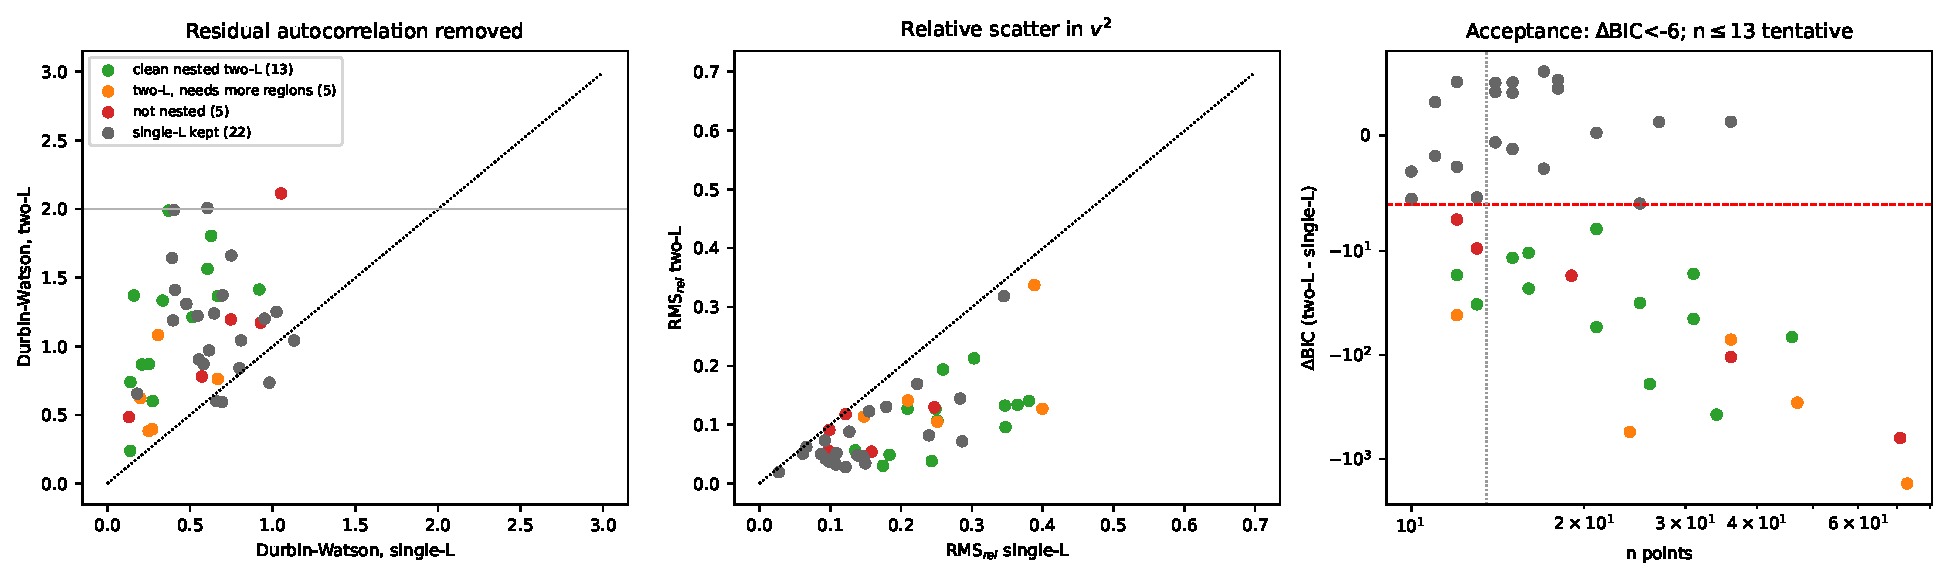
\includegraphics[width=\textwidth]{catB_fig_quality.pdf}\caption{Left: Durbin--Watson statistic before and after the two-L fit (2 = uncorrelated residuals). Middle: relative RMS in $v^2$, single-L versus two-L. Right: $\Delta$BIC versus number of points; acceptance threshold $-6$ (red) and tentative limit $n\le13$ (dotted). Colours: clean nested (green), needs more regions (orange), not nested (red), single-L kept (grey).}\end{figure}
\section{Fit quality of the accepted fits}
\begin{table}[h]\centering\small\caption{Fit-quality statistics (medians), single-L $\to$ two-L.}\begin{tabular}{lrrr}\toprule & Clean nested (13) & Needs more regions (5) & Not nested (5)\\\midrule
$\chi^2_\nu$ & 2.57 $\to$ 0.39 & 9.69 $\to$ 3.48 & 2.98 $\to$ 2.19\\
RMS$_\mathrm{rel}$ & 0.251 $\to$ 0.127 & 0.251 $\to$ 0.127 & 0.122 $\to$ 0.091\\
Durbin--Watson & 0.33 $\to$ 1.33 & 0.27 $\to$ 0.62 & 0.75 $\to$ 1.17\\
$p_\mathrm{runs}<0.05$ after two-L & 7/13 & 4/5 & 4/5\\
$p_\mathrm{runs}<0.05$ after two-L$+\Phi_\mathrm{BH}$ & 5/13 & 4/5 & 3/5\\
$\Delta$BIC (median) & -31.6 & -286.9 & -17.3\\
\bottomrule\end{tabular}\end{table}
\paragraph{Clean nested fits.} The two-L model removes most of the coherent residual. The median RMS$_\mathrm{rel}$ halves, the median $\chi^2_\nu$ drops from 2.57 to 0.39, and the residual sign pattern is broken in all cases (atlas). Residual structure is not fully removed in 7 galaxies (DDO161, NGC0055, NGC0247, NGC7793, UGC04278, UGC07524, UGC12732). Adding the shared offset $\Phi_\mathrm{BH}$ brings $p_\mathrm{runs}$ above 0.05 in DDO 161 and UGC 12732. In the others the remaining pattern is consistent with a further region (virial window) as introduced in the $H_z$ paper; in NGC 7793 it is the declining outer curve. As in category A, $\chi^2_\nu<1$ is common (median 0.39; 7 galaxies with $P(\chi^2\le\chi^2_\mathrm{obs})<0.01$) because SPARC errors are conservative. Shapiro--Wilk rejects normality of the two-L residuals in 2 of 13.

\paragraph{Offset $\Phi_\mathrm{BH}$.} Among the clean fits only IC 2574 strongly prefers the offset ($\Delta\mathrm{BIC}=-7.9$, $\Phi_\mathrm{BH}=23\pm6$\,km$^2$s$^{-2}$). ESO116-G012, NGC 247 and UGC 12732 show positive evidence ($-6<\Delta\mathrm{BIC}<-4.7$; $\Phi_\mathrm{BH}\approx430$, 360 and 950\,km$^2$s$^{-2}$). NGC 247 and UGC 12732 are the two galaxies where the 2018 fit also needed $V_0^2$ (359 and 949), in remarkable agreement.

\paragraph{Needs more regions.} DDO154, NGC1003, NGC2403, NGC5585, UGC03580. The two-L fit improves these enormously (NGC 2403: $\Delta\mathrm{BIC}=-1719$), but $\chi^2_\nu$ stays at 2.8--7.9 and the atlas shows coherent outer residuals. These are three-region (bulge--bar--disk--virial) or three-Lagrangian systems.

\paragraph{Not nested.} NGC3726, NGC4013, UGC02885, UGC06614, UGC06787. Here the optimiser places $R_2$ so that $v^2$ drops by 45--85\% or $M_2<M_1$. In NGC 4013 the inner radius also runs to its lower bound. These are mostly early types or edge-on systems (Sa--Sc; NGC 4013 is edge-on) whose rising--peaked--declining curves are not a bar-in-disk configuration. The statistical gain is real but the two-L parameters have no nested-spiral interpretation, so these galaxies should be moved to category C or D.
\section{Parameter determination}
For the clean nested fits the outer Lagrangian is much better determined than the inner one: median relative errors are 7\% ($M_2$), 5\% ($R_2$, profile) and 1.6\% ($v_{L2}$), against 22\%, 13\% and 5.4\% for $M_1$, $R_1$ and $v_{L1}$. As in category A, each pair is strongly correlated (median $\rho_{M_1R_1}$ = 0.96), and the well-determined quantities are the two asymptotic speeds.

\paragraph{The $R_2$ likelihood.} Fig.~2 shows $\Delta\chi^2(R_2)$. In most galaxies the minimum is sharp and lies between two data radii, so the $\Delta\chi^2\le1$ interval is effectively the gap between neighbouring points and is often asymmetric. In NGC 247 and especially UGC 12732 the profile has several near-equal minima (UGC 12732: four $\Delta\chi^2\le1$ islands between 9.6 and 10.1\,kpc, plus shallow minima down to 5\,kpc). Its $R_2$ is therefore set by the sampling rather than measured, and its grade-II status should be read with that in mind. This sampling dependence is intrinsic to a model with a discontinuity; a smooth transition of width $\sim$ the point spacing would remove it.

\paragraph{Systematics, jackknife, $H_z$.} Distance and inclination systematics exceed the statistical errors (median sys/stat 1.2 for $M_1$, 1.8 for $M_2$, 2.6 for $R_2$) and should be quoted alongside them. Leave-one-out scatter is within 30\% for grade I but larger for several grade II galaxies (ESO116-G012: one point controls $M_1$). Setting $H_z=0$ changes no parameter by more than 1.9\%.
\begin{figure}[h]\centering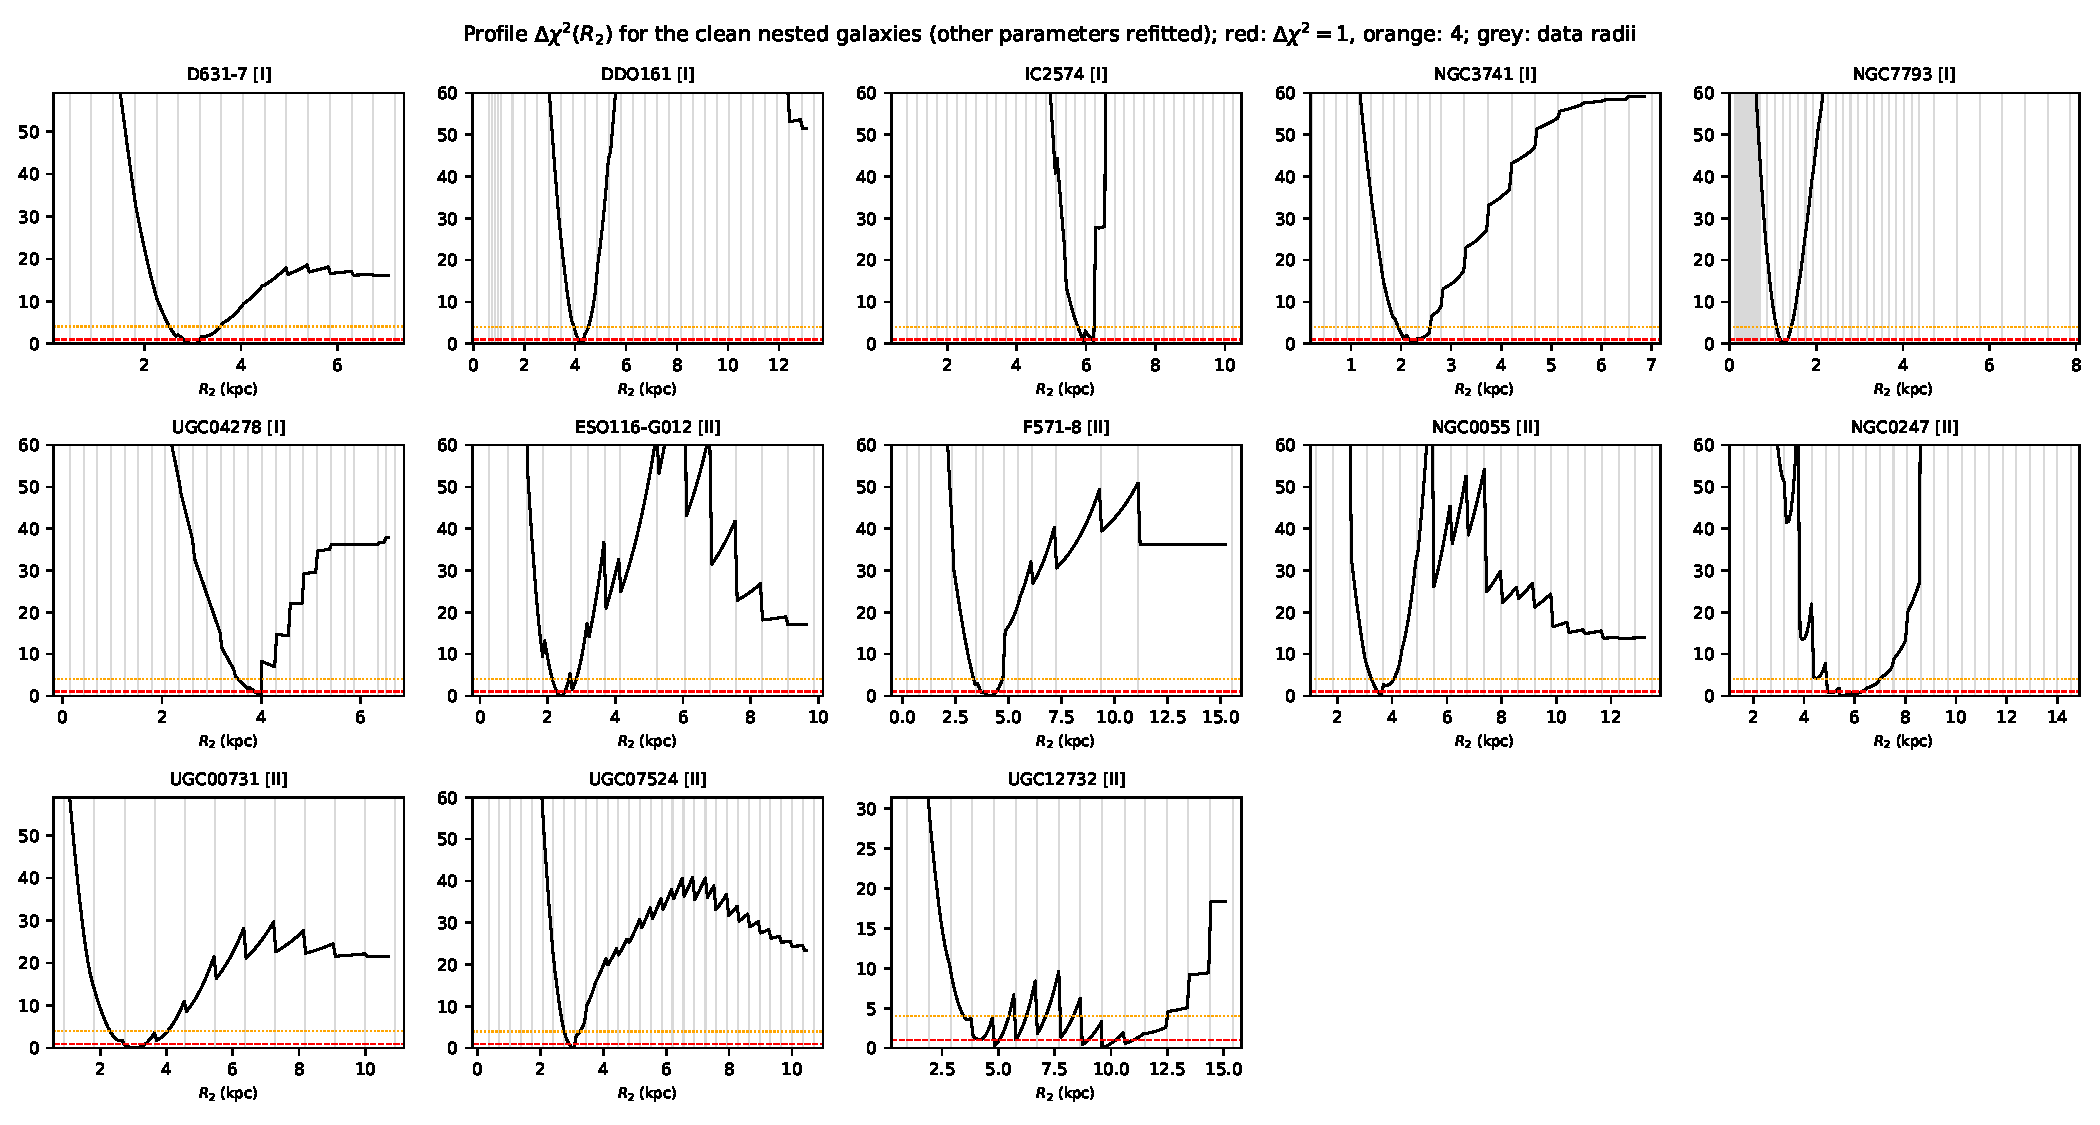
\includegraphics[width=\textwidth]{catB_fig_profiles.pdf}\caption{Profile $\Delta\chi^2(R_2)$ for the 13 clean nested fits. Vertical grey lines are the data radii; the likelihood changes slope at each, so $R_2$ is localised between data points. Multiple minima (NGC 247, UGC 12732) indicate sampling-limited $R_2$.}\end{figure}
\section{Physical consistency}
\begin{itemize}\itemsep0pt
\item \textbf{Seed versus fit.} $R_2/r_{\times1}$ = 1.20 (16--84\%: 1.11--1.85), consistent with the seed factor $1/0.8=1.25$. The residual crossover is a good locator of the Lagrangian reset.
\item \textbf{Nesting.} $R_1/R_2$ = 0.29, $M_2/M_1$ = 8.4 (16--84\%: 6.2--12.7), $v_{L2}/v_{L1}$ = 1.63. The bar zone lies at about $0.3$--$1\,R_2$, and the outer Lagrangian carries about eight times the inner mass.
\item \textbf{Disk scale.} $R_2/R_\mathrm{disk}$ = 1.58 (Spearman $\rho$ = 0.52), so the reset lies about 1--4 disk scale lengths out, where bars and inner rings are found.
\item \textbf{Asymptotic speed.} $v_{L2}$ tracks SPARC $V_\mathrm{flat}$ ($r$ = 0.992, 11 galaxies), with $v_{L2}/V_\mathrm{flat}$ = 1.14. As in category A, the CL curve is still rising at the last measured point.
\item \textbf{Mass.} $M_2/M_\mathrm{bar}$ = 1.06 (16--84\%: 0.61--2.16), $r(\log M_2,\log M_\mathrm{bar})$ = 0.74. The outer Lagrangian mass is comparable to the SPARC baryonic mass.
\item \textbf{Jump at $R_2$.} For the clean fits $v^2$ changes by -0.12 to +0.76 (median +0.19) across $R_2$. No data point lies at $R_2$, so the jump size is a model feature that the data do not constrain directly.
\item \textbf{Morphology.} The clean fits are all late types (Sc--Im: Sc 1, Sd 4, Sm 4, Im 4), and 10 of 13 are Q=1. The non-nested and multi-region cases include all the early types.
\end{itemize}
\begin{figure}[h]\centering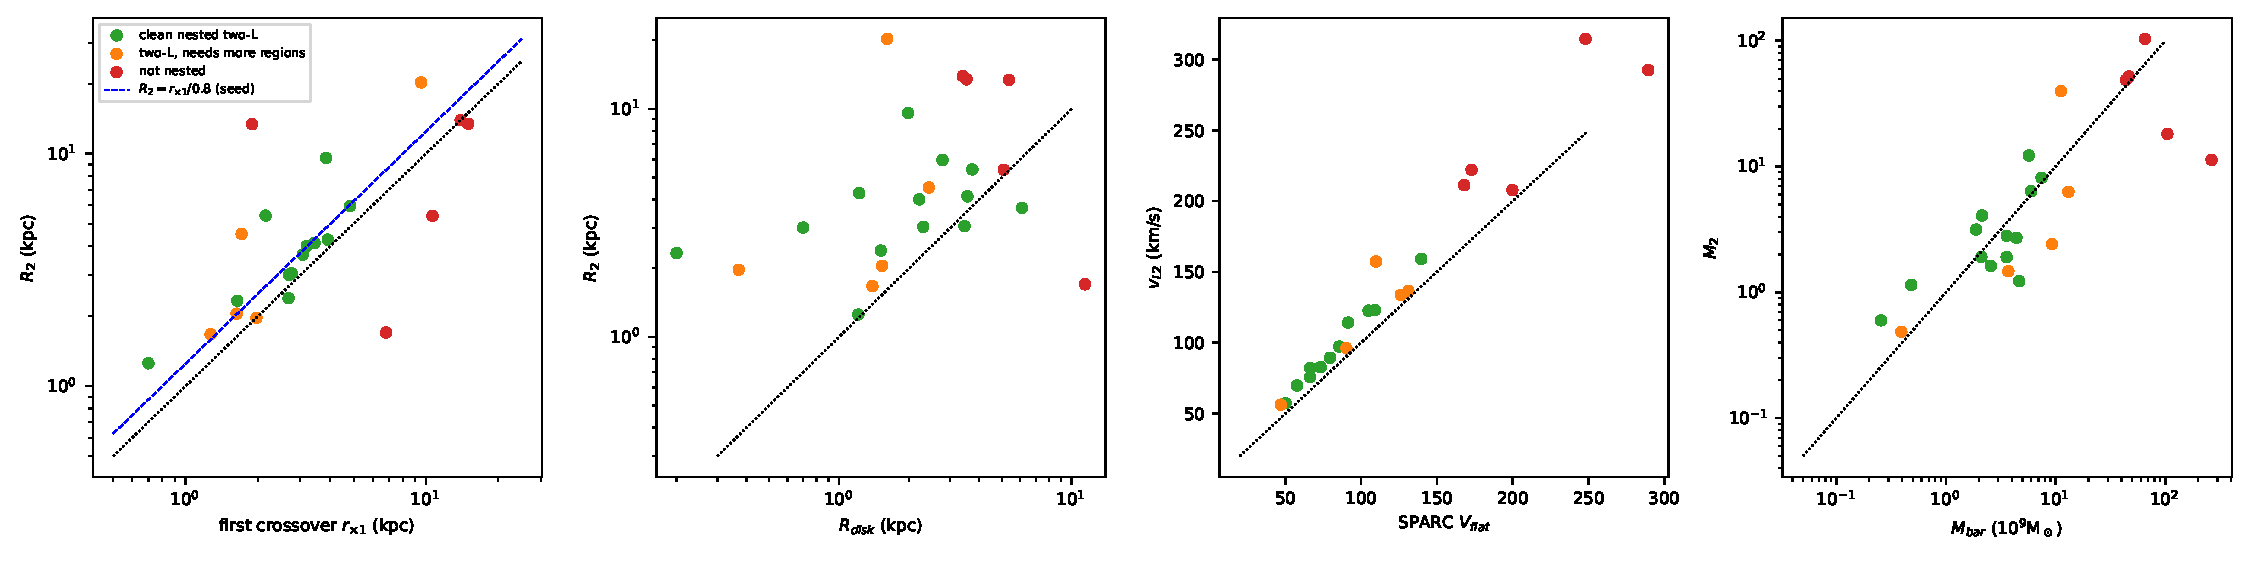
\includegraphics[width=\textwidth]{catB_fig_physics.pdf}\caption{Accepted fits. Left to right: $R_2$ versus first residual crossover (dashed: seed relation); $R_2$ versus $R_\mathrm{disk}$; $v_{L2}$ versus SPARC $V_\mathrm{flat}$; $M_2$ versus $M_\mathrm{bar}$. Colours as in Fig.~1.}\end{figure}
\section{Assessment}
\textbf{Detection works.} The wave screen plus BIC selects 13 clean nested two-L galaxies. All are late types with Q mostly 1. They include 8 of the 13 galaxies identified as double fits by hand in 2018, and the automated $R_2$ agrees with the crossover radius. In these galaxies the two-L model is preferred by $\Delta\mathrm{BIC}$ from $-8$ to $-374$, removes the coherent residual wave, and yields an outer Lagrangian ($v_{L2}$, $M_2$) that matches independent photometric and kinematic scales.

\textbf{Grades.} Grade I (D631--7, DDO161, IC2574, NGC3741, NGC7793, UGC04278) is the robust core, with every parameter determined to within 30\% and each zone sampled. Grade II (ESO116--G012, F571--8, NGC0055, NGC0247, UGC00731, UGC07524, UGC12732) has well-determined asymptotic speeds, but one parameter is weakly constrained or influenced by one point. UGC 12732 and NGC 247 have sampling-limited $R_2$.

\textbf{Limits.} (i) $\Delta$BIC accepts any statistically better fit, so physical screening (N, M) is essential. 10 of the 23 accepted fits are not clean nested spirals. (ii) $R_2$ is localised only to the gap between data points, and the size of the $v^2$ jump is unconstrained. (iii) Residual structure remains in about half of the clean fits, mostly in the outer disk, which motivates the virial-window extension. (iv) For $n\lesssim 15$ the $-6$ threshold is conservative, so the seven galaxies with $-6\le\Delta\mathrm{BIC}<-2$ remain undecided.

\clearpage\begin{landscape}{\scriptsize\setlength{\tabcolsep}{3pt}
\begin{longtable}{lllrrrrrrrrll}
\caption{All category-B galaxies: single-L fit, wave statistics and model-selection outcome. $\dagger$ = 2018 double fit.}\\\toprule
Galaxy & Type & Q & $n$ & $\chi^2_{\nu,1L}$ & RMS$_{1L}$ & $p_\mathrm{runs}$ & $A_{+-+}$ & $r_{\times1}$ & $\chi^2_{\nu,2L}$ & $\Delta$BIC & Outcome & Grade\\\midrule\endfirsthead
\toprule Galaxy & Type & Q & $n$ & $\chi^2_{\nu,1L}$ & RMS$_{1L}$ & $p_\mathrm{runs}$ & $A_{+-+}$ & $r_{\times1}$ & $\chi^2_{\nu,2L}$ & $\Delta$BIC & Outcome & Grade\\\midrule\endhead\bottomrule\endfoot
NGC2403 & Scd & 1 & 73 & 32.04 & 0.251 & 3.6e-13 & 0.96 & 1.27 & 7.93 & -1719.3 & two-L, needs more regions & IM\\
UGC06787 & Sab & 2 & 71 & 25.98 & 0.247 & 1.7e-13 & 0.87 & 1.89 & 17.26 & -627.4 & not nested & N\\
NGC5585 & Sd & 1 & 24 & 28.93 & 0.400 & 1.1e-04 & 0.92 & 1.63 & 4.05 & -549.1 & two-L, needs more regions & IIM\\
IC2574$^\dagger$ & Sm & 2 & 34 & 13.13 & 0.251 & 6.8e-06 & 0.94 & 4.84 & 1.30 & -374.1 & clean nested two-L & I\\
UGC03580 & Sa & 2 & 47 & 9.69 & 0.388 & 1.2e-10 & 1.00 & 1.71 & 3.29 & -286.9 & two-L, needs more regions & IM\\
NGC0247$^\dagger$ & Sd & 2 & 26 & 8.58 & 0.243 & 8.7e-06 & 1.00 & 2.15 & 0.43 & -189.9 & clean nested two-L & II\\
NGC4013 & Sb & 2 & 36 & 5.52 & 0.122 & 2.0e-07 & 0.92 & 14.98 & 2.36 & -104.9 & not nested & N\\
NGC1003 & Scd & 1 & 36 & 4.91 & 0.148 & 1.0e-04 & 0.92 & 9.54 & 2.77 & -71.2 & two-L, needs more regions & IM\\
NGC7793 & Sd & 1 & 46 & 2.57 & 0.303 & 4.4e-08 & 0.93 & 0.70 & 0.90 & -67.5 & clean nested two-L & I\\
NGC3741$^\dagger$ & Im & 1 & 21 & 3.52 & 0.365 & 7.5e-05 & 1.00 & 1.64 & 0.39 & -54.0 & clean nested two-L & I\\
DDO161$^\dagger$ & Im & 1 & 31 & 2.15 & 0.348 & 9.0e-05 & 0.90 & 3.90 & 0.38 & -45.1 & clean nested two-L & I\\
DDO154 & Im & 2 & 12 & 7.43 & 0.210 & 3.8e-02 & 0.83 & 1.97 & 3.48 & -41.6 & two-L, needs more regions (tent.) & IIM\\
F571--8$^\dagger$ & Sc & 1 & 13 & 3.79 & 0.347 & 4.6e-03 & 1.00 & 3.44 & 0.44 & -32.6 & clean nested two-L (tent.) & II\\
UGC04278$^\dagger$ & Sd & 1 & 25 & 1.97 & 0.381 & 1.4e-05 & 1.00 & 3.19 & 0.35 & -31.6 & clean nested two-L & I\\
UGC12732$^\dagger$ & Sm & 1 & 16 & 2.81 & 0.209 & 9.9e-04 & 1.00 & 3.84 & 0.90 & -23.0 & clean nested two-L & II\\
UGC02885 & Sc & 1 & 19 & 2.03 & 0.098 & 4.8e-03 & 0.89 & 6.82 & 0.75 & -17.3 & not nested & N\\
UGC00731 & Im & 1 & 12 & 2.34 & 0.175 & 8.3e-03 & 1.00 & 2.73 & 0.16 & -17.1 & clean nested two-L (tent.) & II\\
UGC07524 & Sm & 1 & 31 & 1.07 & 0.249 & 6.7e-05 & 0.94 & 2.76 & 0.28 & -16.6 & clean nested two-L & II\\
ESO116--G012 & Sd & 1 & 15 & 2.57 & 0.259 & 7.1e-03 & 1.00 & 2.68 & 1.49 & -11.7 & clean nested two-L & II\\
D631--7$^\dagger$ & Im & 1 & 16 & 1.33 & 0.184 & 2.3e-03 & 1.00 & 2.69 & 0.22 & -10.4 & clean nested two-L & I\\
UGC06614 & Sa & 1 & 13 & 1.62 & 0.158 & 4.6e-03 & 0.92 & 10.64 & 0.33 & -9.8 & not nested (tent.) & N\\
NGC0055 & Sm & 2 & 21 & 1.04 & 0.135 & 1.3e-04 & 1.00 & 3.07 & 0.33 & -8.1 & clean nested two-L & II\\
NGC3726 & Sc & 2 & 12 & 2.98 & 0.099 & 3.8e-02 & 0.83 & 13.94 & 2.19 & -7.3 & not nested (tent.) & N\\
NGC3109$^\dagger$ & Sm & 1 & 25 & 0.78 & 0.127 & 2.6e-04 & 0.96 & 2.06 & 0.26 & -5.9 & single-L kept & --\\
UGC07323 & Sdm & 1 & 10 & 1.68 & 0.284 & 3.6e-02 & 1.00 & 2.91 & 0.54 & -5.6 & single-L kept & --\\
NGC3972$^\dagger$ & Sbc & 1 & 10 & 1.42 & 0.138 & 2.2e-02 & 1.00 & 2.61 & 0.20 & -5.5 & single-L kept & --\\
UGC07125 & Sm & 1 & 13 & 1.15 & 0.150 & 7.2e-03 & 1.00 & 4.33 & 0.23 & -5.4 & single-L kept & --\\
UGC07399 & Sdm & 1 & 10 & 1.29 & 0.098 & 2.5e-02 & 0.90 & 1.84 & 0.43 & -3.1 & single-L kept & --\\
UGC06446$^\dagger$ & Sd & 1 & 17 & 0.67 & 0.147 & 4.3e-03 & 0.94 & 1.74 & 0.11 & -2.9 & single-L kept & --\\
NGC4010 & Sd & 2 & 12 & 1.69 & 0.239 & 3.8e-02 & 0.83 & 3.50 & 1.15 & -2.7 & single-L kept & --\\
UGC05829$^\dagger$ & Im & 2 & 11 & 0.83 & 0.286 & 1.3e-02 & 1.00 & 3.14 & 0.12 & -1.8 & single-L kept & --\\
ESO079--G014 & Sbc & 1 & 15 & 1.12 & 0.345 & 9.3e-03 & 0.93 & 5.65 & 0.72 & -1.2 & single-L kept & --\\
NGC4214 & Im & 2 & 14 & 0.53 & 0.122 & 9.7e-03 & 0.93 & 1.04 & 0.04 & -0.6 & single-L kept & --\\
NGC0100 & Scd & 1 & 21 & 0.37 & 0.146 & 2.5e-03 & 0.90 & 2.51 & 0.07 & 0.2 & single-L kept & --\\
NGC2976 & Sc & 2 & 27 & 0.47 & 0.155 & 1.3e-02 & 0.85 & 1.01 & 0.28 & 1.1 & single-L kept & --\\
UGCA444 & Im & 2 & 36 & 0.26 & 0.223 & 7.6e-06 & 0.97 & 0.97 & 0.09 & 1.2 & single-L kept & --\\
UGC08550 & Sd & 1 & 11 & 0.68 & 0.061 & 1.3e-02 & 1.00 & 1.47 & 0.60 & 2.9 & single-L kept & --\\
UGC12632 & Sm & 1 & 15 & 0.28 & 0.179 & 1.8e-03 & 1.00 & 3.55 & 0.18 & 3.7 & single-L kept & --\\
F574--1 & Sd & 1 & 14 & 0.16 & 0.109 & 2.9e-03 & 1.00 & 2.35 & 0.03 & 3.7 & single-L kept & --\\
F568--3 & Sd & 1 & 18 & 0.19 & 0.092 & 1.4e-02 & 0.94 & 5.39 & 0.09 & 4.0 & single-L kept & --\\
F579--V1 & Sc & 1 & 14 & 0.10 & 0.108 & 2.7e-03 & 0.93 & 2.11 & 0.04 & 4.5 & single-L kept & --\\
KK98--251 & Im & 2 & 15 & 0.18 & 0.066 & 1.3e-02 & 0.93 & 1.24 & 0.13 & 4.6 & single-L kept & --\\
F568--1 & Sc & 1 & 12 & 0.05 & 0.094 & 7.7e-03 & 1.00 & 3.08 & 0.02 & 4.6 & single-L kept & --\\
NGC5005 & Sbc & 1 & 18 & 0.20 & 0.087 & 1.1e-03 & 1.00 & 1.47 & 0.16 & 4.8 & single-L kept & --\\
UGC08286 & Scd & 1 & 17 & 0.15 & 0.028 & 1.9e-02 & 0.94 & 1.42 & 0.16 & 5.5 & single-L kept & --\\
\end{longtable}
\begin{longtable}{llrlllllrrrr}
\caption{Accepted two-L fits: parameters. $R$ in kpc, $M$ in $10^9M_\odot$, $v_L$ in km\,s$^{-1}$. $R_1,M_1$: statistical $\pm$ systematic; $R_2,M_2$: profile $\Delta\chi^2\le1$ interval, and systematic in brackets. Jump = fractional $v^2$ change at $R_2$. $\Phi_\mathrm{BH}$ from the two-L$+\Phi_\mathrm{BH}$ fit.}\\\toprule
Galaxy & Grade & $n$ & $R_1$ & $M_1$ & $R_2$ & $M_2$ & $v_{L1}$ & $v_{L2}$ & zones & jump & $\Phi_\mathrm{BH}$\\\midrule\endfirsthead
\toprule Galaxy & Grade & $n$ & $R_1$ & $M_1$ & $R_2$ & $M_2$ & $v_{L1}$ & $v_{L2}$ & zones & jump & $\Phi_\mathrm{BH}$\\\midrule\endhead\bottomrule\endfoot
IC2574 & I & 34 & $2.55\pm0.054\pm0.13$ & $0.518\pm0.021\pm0.037$ & $5.97^{+0}_{-0.013}$ [0.31] & $3.16^{+0.0097}_{-0.015}$ [0.22] & $50.9\pm0.53$ & $82.1\pm0.48$ & 7/11/16 & +0.20 & $23\pm6.2$\\
NGC7793 & I & 46 & $0.338\pm0.036\pm0.017$ & $0.134\pm0.026\pm0.031$ & $1.25^{+0.054}_{-0.052}$ [0.062] & $1.23^{+0.08}_{-0.074}$ [0.28] & $71.6\pm3.4$ & $112.4\pm2.4$ & 7/14/25 & +0.00 & $-93\pm1.5e+02$\\
NGC3741 & I & 21 & $0.485\pm0.065\pm0.026$ & $0.0397\pm0.0081\pm0.0027$ & $2.33^{+0}_{-0.13}$ [0.12] & $0.599^{+0.00027}_{-0.055}$ [0.041] & $32.5\pm1.4$ & $57.4\pm0.89$ & 2/7/12 & +0.21 & $128\pm65$\\
DDO161 & I & 31 & $1.26\pm0.16\pm0.38$ & $0.196\pm0.044\pm0.061$ & $4.27^{+0.017}_{-0.15}$ [1.3] & $1.92^{+0.012}_{-0.099}$ [0.59] & $44.7\pm2.5$ & $75.7\pm0.72$ & 5/6/20 & +0.18 & $156\pm92$\\
UGC04278 & I & 25 & $1.03\pm0.14\pm0.31$ & $0.238\pm0.053\pm0.071$ & $4.01^{+0}_{-0.094}$ [1.2] & $4.08^{+0.03}_{-0.2}$ [1.2] & $54.5\pm2.7$ & $114.2\pm2.3$ & 4/10/11 & +0.76 & $16\pm56$\\
D631--7 & I & 16 & $1.43\pm0.16\pm0.033$ & $0.242\pm0.056\pm0.015$ & $3.02^{+0.12}_{-0.2}$ [0.07] & $1.15^{+0.092}_{-0.14}$ [0.071] & $46.7\pm2.9$ & $69.8\pm2.4$ & 3/3/10 & +0.08 & $1\pm33$\\
NGC0247 & II & 26 & $1.59\pm0.032\pm0.081$ & $0.835\pm0.031\pm0.048$ & $5.42^{+0.77}_{-0}$ [0.28] & $6.37^{+1.7}_{-0}$ [0.37] & $82.2\pm0.79$ & $122.7\pm4.1$ & 1/8/17 & -0.08 & $359\pm1.3e+02$\\
F571--8 & II t & 13 & $1.14\pm0.15\pm0.23$ & $0.687\pm0.17\pm0.14$ & $4.13^{+0.19}_{-0.41}$ [0.83] & $8.16^{+0.62}_{-1.3}$ [1.6] & $88.2\pm5.5$ & $159.2\pm4.1$ & 2/4/7 & +0.32 & $99\pm1.8e+02$\\
UGC12732 & II & 16 & $1.79\pm0.18\pm0.56$ & $0.978\pm0.14\pm0.37$ & $9.6^{+0.55}_{-0}$ [2.9] & $12.2^{+1.5}_{-0.014}$ [4.5] & $83.8\pm2.1$ & $127.5\pm2$ & 1/9/6 & -0.12 & $955\pm2.6e+02$\\
UGC00731 & II t & 12 & $1.02\pm0.12\pm0.31$ & $0.26\pm0.057\pm0.079$ & $3.04^{+0.32}_{-0.3}$ [0.9] & $1.62^{+0.26}_{-0.23}$ [0.49] & $57.2\pm3.3$ & $82.8\pm2.4$ & 1/2/9 & -0.10 & $411\pm4.5e+02$\\
UGC07524 & II & 31 & $1.06\pm0.14\pm0.054$ & $0.228\pm0.052\pm0.024$ & $3.06^{+0.011}_{-0.12}$ [0.15] & $1.91^{+0.01}_{-0.11}$ [0.2] & $52.5\pm2.9$ & $89.4\pm1.4$ & 3/5/23 & +0.25 & $188\pm84$\\
ESO116--G012 & II & 15 & $0.927\pm0.13\pm0.28$ & $0.412\pm0.11\pm0.12$ & $2.39^{+0.083}_{-0.1}$ [0.71] & $2.82^{+0.14}_{-0.17}$ [0.84] & $75.6\pm5.4$ & $123.1\pm1.6$ & 2/2/11 & +0.19 & $432\pm1.4e+02$\\
NGC0055 & II & 21 & $1.52\pm0.25\pm0.079$ & $0.381\pm0.11\pm0.021$ & $3.68^{+0}_{-0.16}$ [0.19] & $2.72^{+0}_{-0.2}$ [0.15] & $56.9\pm3.8$ & $97.3\pm0.77$ & 1/3/17 & +0.34 & $593\pm2.1e+02$\\
\midrule
NGC5585 & IIM & 24 & $0.234\pm0.015\pm0.07$ & $0.0305\pm0.003\pm0.0093$ & $2.05^{+0}_{-0}$ [0.62] & $1.47^{+0.0076}_{-0}$ [0.45] & $41.0\pm0.79$ & $96.0\pm0.59$ & 1/9/14 & +0.98 & $17\pm52$\\
DDO154 & IIM t & 12 & $1.2\pm0.13\pm0.059$ & $0.18\pm0.047\pm0.012$ & $1.97^{+0.0054}_{-0}$ [0.098] & $0.486^{+0.0021}_{-4e-05}$ [0.033] & $44.0\pm3.4$ & $56.3\pm0.13$ & 2/2/8 & -0.09 & $128\pm43$\\
NGC2403 & IM & 73 & $0.495\pm0.011\pm0.025$ & $0.355\pm0.014\pm0.025$ & $1.67^{+0}_{-0}$ [0.085] & $2.42^{+0}_{-0}$ [0.17] & $96.2\pm0.84$ & $136.5\pm0.11$ & 4/12/57 & -0.16 & $1028\pm90$\\
UGC03580 & IM & 47 & $1.01\pm0.042\pm0.27$ & $0.824\pm0.052\pm0.23$ & $4.52^{+0.019}_{-0}$ [1.1] & $6.31^{+0.033}_{-0.0032}$ [1.6] & $102.6\pm1.3$ & $133.8\pm0.44$ & 8/21/18 & -0.34 & $3601\pm2.4e+02$\\
NGC1003 & IM & 36 & $2.12\pm0.12\pm0.69$ & $1.8\pm0.12\pm0.59$ & $20.3^{+0.077}_{-0}$ [6.1] & $39.8^{+0.15}_{-0.15}$ [12] & $104.4\pm0.74$ & $157.3\pm0.97$ & 2/22/12 & -0.19 & $3370\pm5.5e+02$\\
\midrule
UGC06787 & N & 71 & $0.124\pm0.025\pm0.031$ & $0.58\pm0.12\pm0.15$ & $13.4^{+0}_{-0}$ [3.3] & $104^{+0}_{-0}$ [26] & $245.4\pm0.48$ & $314.6\pm0.68$ & 1/51/19 & -0.45 & $24405\pm1.6e+04$\\
NGC4013 & N & 36 & $0.02\pm0.84\pm0.0028$ & $0.0577\pm2.4\pm0.008$ & $13.5^{+0}_{-0}$ [1.9] & $52^{+0}_{-0}$ [7.2] & $192.9\pm6$ & $222.1\pm1.4$ & 0/12/24 & -0.56 & $19890\pm\mathrm{n/a}$\\
UGC02885 & N & 19 & $0.863\pm\mathrm{n/a}\pm0.039$ & $9.42\pm\mathrm{n/a}\pm0.6$ & $1.7^{+0}_{-0}$ [0.17] & $11.3^{+0}_{-0.006}$ [1.3] & $375.2\pm\mathrm{n/a}$ & $292.6\pm\mathrm{n/a}$ & 0/1/18 & -0.69 & $73141\pm3.4e+03$\\
UGC06614 & N t & 13 & $4.28\pm2e+07\pm0.56$ & $65.8\pm9.1e+08\pm22$ & $5.41^{+0.77}_{-0.92}$ [0.54] & $18.2^{+3.6}_{-3.9}$ [6.3] & $445.0\pm2.1e+09$ & $207.8\pm7.1$ & 1/0/12 & -0.85 & $29531\pm1.3e+05$\\
NGC3726 & N t & 12 & $3.57\pm0.27\pm0.5$ & $8.99\pm1\pm1.3$ & $13.9^{+0.13}_{-0}$ [1.9] & $48.8^{+0.32}_{-0.47}$ [7.2] & $180.0\pm4.1$ & $211.3\pm4.2$ & 1/6/5 & -0.45 & $6415\pm3.6e+03$\\
\end{longtable}
\begin{longtable}{lrrrrrrrrrrrr}
\caption{Accepted two-L fits: goodness of fit. Subscripts 1, 2, 3 = single-L, two-L, two-L$+\Phi_\mathrm{BH}$. $P_<=P(\chi^2_2\le\chi^2_\mathrm{obs})$; jk = largest relative leave-one-out scatter of the four parameters.}\\\toprule
Galaxy & $\chi^2_{\nu1}$ & $\chi^2_{\nu2}$ & $\chi^2_{\nu3}$ & BIC$_1$ & BIC$_2$ & BIC$_3$ & RMS$_2$ & $p_\mathrm{runs,2}$ & $p_\mathrm{runs,3}$ & DW$_2$ & $P_<$ & jk\\\midrule\endfirsthead
\toprule Galaxy & $\chi^2_{\nu1}$ & $\chi^2_{\nu2}$ & $\chi^2_{\nu3}$ & BIC$_1$ & BIC$_2$ & BIC$_3$ & RMS$_2$ & $p_\mathrm{runs,2}$ & $p_\mathrm{runs,3}$ & DW$_2$ & $P_<$ & jk\\\midrule\endhead\bottomrule\endfoot
IC2574 & 13.13 & 1.30 & 0.95 & 427.1 & 53.0 & 45.2 & 0.107 & 0.223 & 0.348 & 1.41 & 0.873 & 0.17\\
NGC7793 & 2.57 & 0.90 & 0.92 & 120.7 & 53.3 & 56.7 & 0.213 & 0.002 & 0.001 & 0.24 & 0.350 & 0.20\\
NGC3741 & 3.52 & 0.39 & 0.30 & 72.9 & 18.8 & 20.0 & 0.134 & 0.148 & 0.148 & 1.37 & 0.012 & 0.01\\
DDO161 & 2.15 & 0.38 & 0.32 & 69.2 & 24.1 & 25.6 & 0.096 & 0.001 & 0.062 & 0.60 & 0.002 & 0.19\\
UGC04278 & 1.97 & 0.35 & 0.36 & 51.8 & 20.2 & 23.3 & 0.141 & 0.000 & 0.001 & 0.74 & 0.003 & 0.16\\
D631--7 & 1.33 & 0.22 & 0.24 & 24.2 & 13.8 & 16.6 & 0.049 & 0.150 & 0.150 & 1.33 & 0.003 & 0.21\\
NGC0247 & 8.58 & 0.43 & 0.07 & 212.4 & 22.5 & 17.8 & 0.038 & 0.005 & 0.008 & 1.99 & 0.010 & 0.12\\
F571--8 & 3.79 & 0.44 & 0.46 & 46.9 & 14.2 & 16.5 & 0.132 & 0.239 & 0.394 & 1.56 & 0.086 & 0.47\\
UGC12732 & 2.81 & 0.90 & 0.24 & 44.9 & 21.9 & 16.5 & 0.127 & 0.021 & 0.065 & 0.87 & 0.452 & 0.23\\
UGC00731 & 2.34 & 0.16 & 0.17 & 28.4 & 11.3 & 13.6 & 0.030 & 0.272 & 0.541 & 1.37 & 0.005 & 0.30\\
UGC07524 & 1.07 & 0.28 & 0.17 & 38.0 & 21.4 & 21.5 & 0.127 & 0.010 & 0.035 & 0.87 & 0.000 & 0.30\\
ESO116--G012 & 2.57 & 1.49 & 0.77 & 38.8 & 27.2 & 21.2 & 0.194 & 0.092 & 0.215 & 1.80 & 0.871 & 2.28\\
NGC0055 & 1.04 & 0.33 & 0.23 & 25.9 & 17.8 & 18.9 & 0.056 & 0.007 & 0.025 & 1.21 & 0.004 & 0.63\\
\midrule
NGC5585 & 28.93 & 4.05 & 4.37 & 642.9 & 93.8 & 98.8 & 0.127 & 0.002 & 0.002 & 1.08 & 1.000 & 0.26\\
DDO154 & 7.43 & 3.48 & 3.10 & 79.3 & 37.7 & 34.1 & 0.141 & 0.272 & 0.541 & 0.76 & 0.999 & 0.35\\
NGC2403 & 32.04 & 7.93 & 7.10 & 2283.4 & 564.2 & 504.3 & 0.105 & 0.000 & 0.000 & 0.62 & 1.000 & 0.22\\
UGC03580 & 9.69 & 3.29 & 1.51 & 443.6 & 156.7 & 82.8 & 0.337 & 0.000 & 0.000 & 0.40 & 1.000 & 0.19\\
NGC1003 & 4.91 & 2.77 & 1.02 & 174.2 & 103.0 & 49.6 & 0.114 & 0.000 & 0.002 & 0.38 & 1.000 & 0.15\\
\midrule
UGC06787 & 25.98 & 17.26 & 11.01 & 1800.9 & 1173.5 & 748.0 & 0.129 & 0.000 & 0.000 & 0.78 & 1.000 & 0.41\\
NGC4013 & 5.52 & 2.36 & 0.48 & 194.8 & 90.0 & 32.7 & 0.118 & 0.000 & 0.000 & 0.48 & 1.000 & 0.08\\
UGC02885 & 2.03 & 0.75 & 1.18 & 40.3 & 23.1 & 31.2 & 0.056 & 0.017 & 0.019 & 1.17 & 0.267 & 0.68\\
UGC06614 & 1.62 & 0.33 & 0.22 & 23.0 & 13.2 & 14.6 & 0.054 & 0.007 & 0.197 & 1.20 & 0.033 & 0.43\\
NGC3726 & 2.98 & 2.19 & 1.94 & 34.7 & 27.4 & 26.0 & 0.091 & 0.409 & 0.338 & 2.11 & 0.975 & 0.21\\
\end{longtable}}\end{landscape}
\section*{Atlas 1: accepted two-L fits with residuals}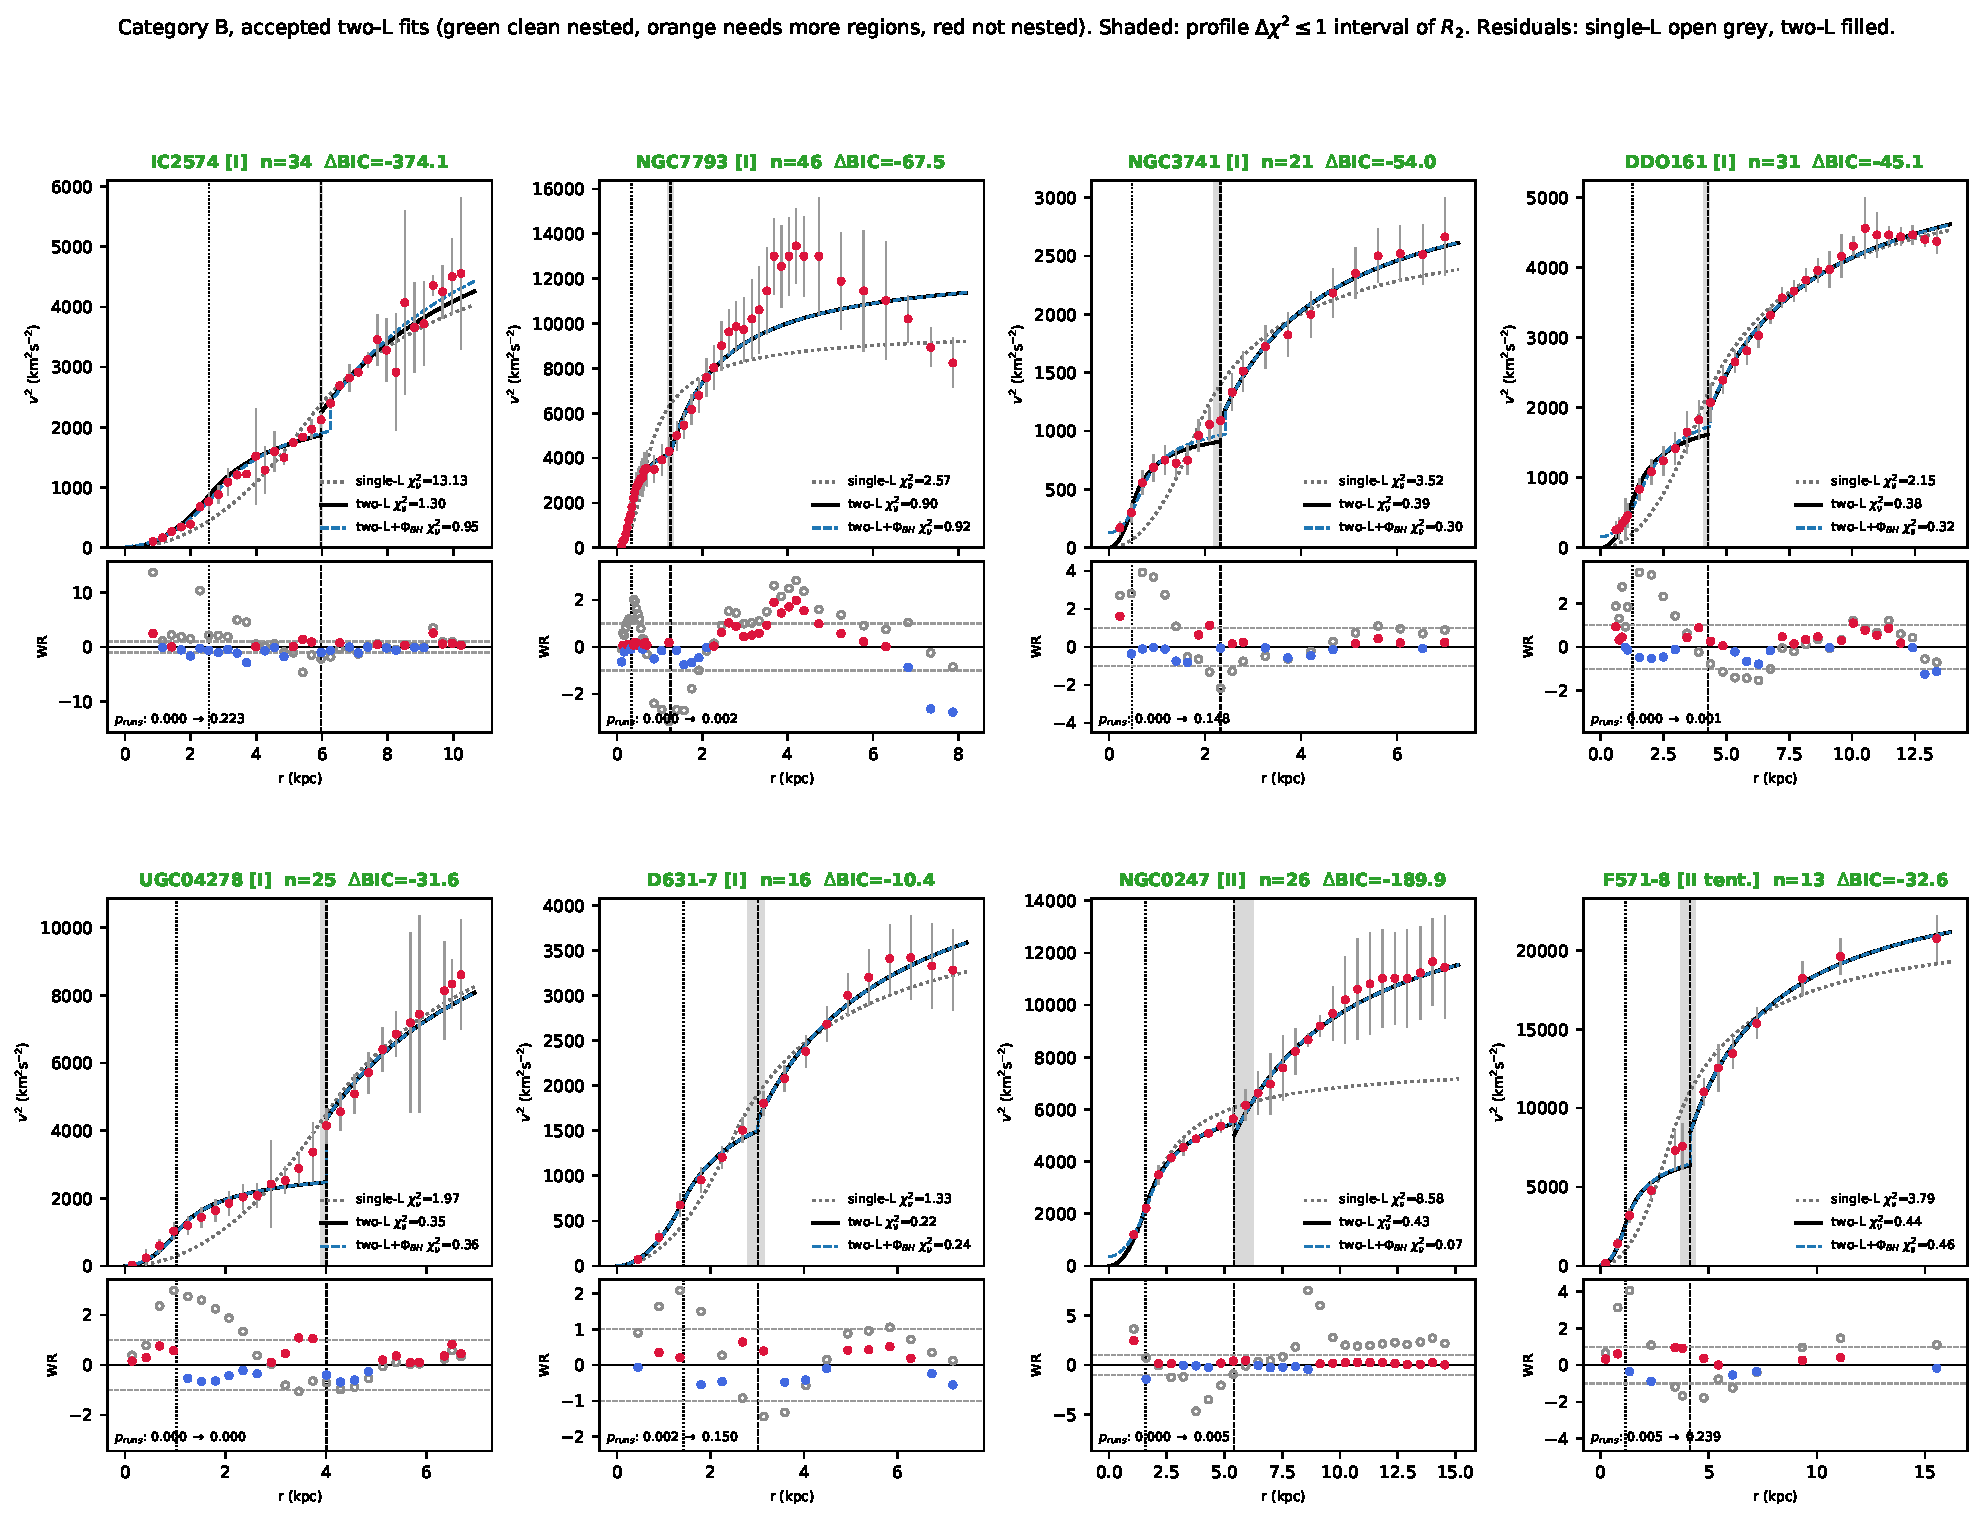
\includepdf[pages=-,landscape=true,scale=0.95]{catB_atlas_accepted.pdf}
\section*{Atlas 2: category-B galaxies with single-L kept}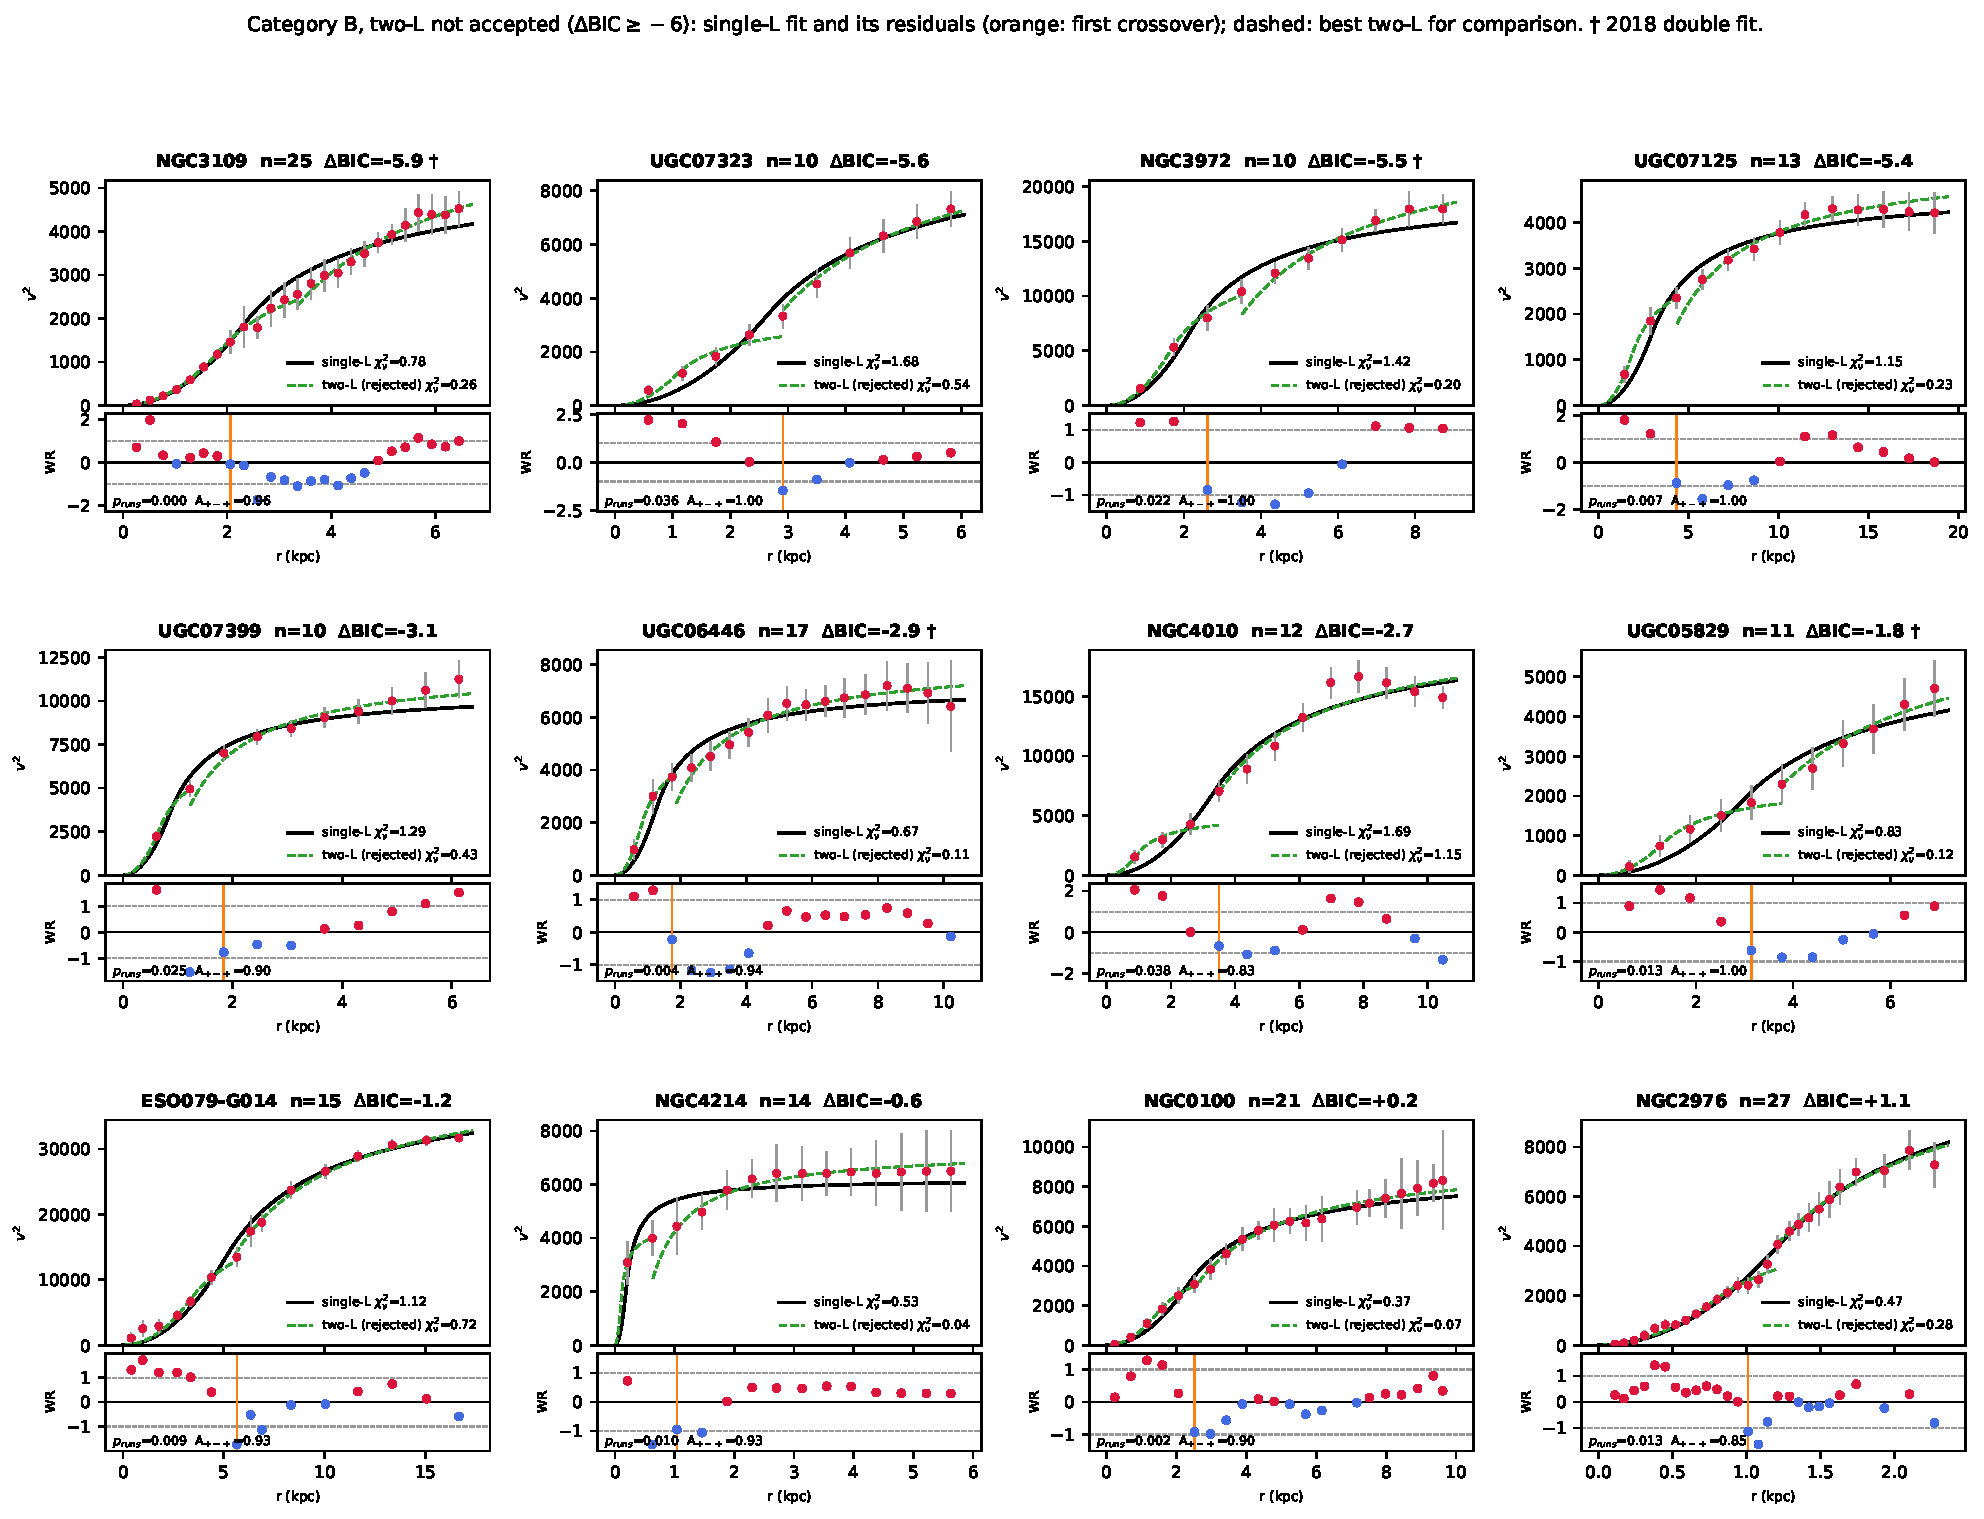
\includepdf[pages=-,landscape=true,scale=0.95]{catB_atlas_rejected.pdf}
\end{document}